\documentclass[11pt,a4paper]{article}
\usepackage[utf8]{inputenc}
\usepackage[T1]{fontenc}
\usepackage[spanish]{babel}
\spanishplainpercent
\usepackage[a4paper,top=4cm,bottom=2.5cm,left=2.5cm,right=2.5cm,headheight=3cm,headsep=.8cm]{geometry}
\usepackage{graphicx,amsmath,amssymb,booktabs,array,siunitx,multirow,float,caption,subcaption}
\usepackage[table]{xcolor}
\usepackage{fancyhdr,lastpage,enumitem,microtype}
\microtypesetup{expansion=false}
\usepackage[colorlinks=true,linkcolor=blue!50!black,urlcolor=blue!50!black,citecolor=blue!50!black]{hyperref}
\graphicspath{{./imagenes/}}
\sisetup{output-decimal-marker={,},group-separator={.}}
\captionsetup{font=small,labelfont=bf}
\makeatletter
\newcommand{\inputtablerows}[1]{\@@input #1 }
\makeatother

% Datos del informe (plantilla)
\newcommand{\TituloInforme}{Práctica No. 5:}
\newcommand{\NombrePractica}{Análisis de datos de entrada y ajuste de datos a distribuciones de probabilidad}
\newcommand{\NombreUniversidad}{Universidad de los Llanos}
\newcommand{\NombreFacultad}{Facultad de Ciencias Básicas e Ingenierías}
\newcommand{\NombrePrograma}{Programa de Ingeniería de Sistemas}
\newcommand{\NombreCurso}{Simulación Computacional}
\newcommand{\TipoDocumento}{Informe de Laboratorio}
\newcommand{\FechaInforme}{Octubre de 2026}
\newcommand{\AlumnoUno}{J. Gregorio Delgado}
\newcommand{\CodUno}{160005010}

\newcommand{\LogoUniversidad}{%
 \IfFileExists{../logo.png}
 {
\includegraphics[width=3cm,height=2.7cm,keepaspectratio]{../logo.png}}
 {\colorbox{gray!15}{\parbox[c][2.4cm][c]{3cm}{\centering\footnotesize Logo institucional}}}}
\pagestyle{fancy}\fancyhf{}\renewcommand{\headrulewidth}{0pt}
\fancyhead[L]{\parbox[c][2.8cm][c]{3.2cm}{\centering\LogoUniversidad}}
\fancyhead[C]{\parbox[c][2.8cm][c]{\dimexpr(\textwidth-4cm)/2\relax}{\centering\footnotesize
 \textbf{\MakeUppercase{\NombreUniversidad}}\\[2pt]Facultad de Ciencias Básicas e Ingenierías}}
\fancyhead[R]{\parbox[c][2.8cm][c]{\dimexpr(\textwidth-4cm)/2\relax}{\raggedleft\footnotesize
 Curso: \NombreCurso\\[2pt]\textbf{\TipoDocumento}}}
\fancyfoot[C]{\small Página \thepage\ de \pageref{LastPage}}

\begin{document}
\begin{center}
 {\LARGE\bfseries \TituloInforme}\\[6pt]
 {\normalsize\itshape \NombrePractica}\\[16pt]
 {\large \AlumnoUno\textsuperscript{1}}\\[12pt]
 {\small 1. Código: \CodUno, Ingeniería de Sistemas.}\\[10pt]
 {\small \NombreFacultad. \NombrePrograma.}\\[4pt]
 {\small Fecha: \FechaInforme}
\end{center}

\vspace{.4cm}\noindent\rule{\textwidth}{.6pt}
\begin{abstract}
Se analizaron cuatro muestras de 200 observaciones (A, B, C y D) de procesos estocásticos,
interpretadas como tiempos entre llegadas, siguiendo el capítulo 3 de Banks \cite{banks1998}.
Primero se describieron con estadística descriptiva e histogramas. Después se evaluaron los
supuestos de independencia y estabilidad con correlaciones de retraso, diagramas de dispersión,
patrón de llegadas, conteos por intervalo y media móvil, complementados con pruebas de
Ljung-Box, rachas, Spearman y Kruskal-Wallis. Por último, se ajustaron nueve distribuciones por
máxima verosimilitud y se compararon con SSE, AIC y BIC. B y D son IID y se modelan con una
Exponencial de media 0,205 y una Lognormal ($\sigma=1{,}019$, escala 1,273). A es estacionario
pero autocorrelacionado ($r_1=0{,}52$): su marginal es aproximadamente Normal y se reproduce
con un AR(1) de innovaciones uniformes. C no es estacionario: su media crece linealmente con el
orden de observación y, al normalizar por esa tendencia, los datos son IID exponenciales. La
Gamma que mejor ajusta los datos agregados de C es solo un efecto de mezclar escalas.

\medskip\noindent\textbf{Palabras clave ---} análisis de datos de entrada, IID, autocorrelación,
estacionariedad, bondad de ajuste, máxima verosimilitud, AIC, BIC.
\end{abstract}
\rule{\textwidth}{.6pt}

\section{Objetivos}
\begin{itemize}
 \item Introducir el análisis de datos de entrada en un estudio de simulación a partir de muestras
 de datos de procesos o fenómenos del sistema objeto de estudio.
 \item Identificar si los valores de una muestra se pueden asociar a una variable aleatoria
 independiente (no correlacionada) y estacionaria.
 \item Evaluar la bondad de ajuste de diferentes distribuciones de probabilidad a un conjunto de datos.
 \item Seleccionar la distribución de probabilidad más apropiada y con mejor ajuste para su
 posterior modelado en un estudio de simulación.
\end{itemize}

\section{Consulta previa}
\begin{enumerate}[label=\arabic*.]
 \item \textbf{Estadística descriptiva.} Es la rama de la estadística que resume y presenta un
 conjunto de datos sin hacer inferencias sobre la población. Usa medidas de tendencia central
 (media, mediana, moda), de dispersión (rango, varianza, desviación estándar, rango
 intercuartílico, coeficiente de variación), de posición (percentiles y cuartiles) y de forma
 (asimetría y curtosis), además de tablas de frecuencia y gráficas como el histograma o el
 diagrama de caja. En simulación es el primer paso para sugerir familias de distribuciones
 candidatas \cite[Sec.~3.5]{banks1998}.
 \item \textbf{Asimetría, curtosis y percentiles.} La \emph{asimetría} (\emph{skewness}),
 $g_1=\frac{1}{n}\sum(x_i-\bar x)^3/s^3$, mide la falta de simetría: vale 0 en una
 distribución simétrica, es positiva si la cola derecha es más larga (la media supera a la
 mediana) y negativa en el caso contrario. La \emph{curtosis},
 $g_2=\frac{1}{n}\sum(x_i-\bar x)^4/s^4-3$ (en exceso respecto a la normal), mide el peso de las
 colas: vale 0 para la normal, es positiva en distribuciones con colas pesadas y negativa en
 distribuciones de colas cortas, como la uniforme ($-1{,}2$). El \emph{percentil} $p$ es el
 valor por debajo del cual queda el $p\,\%$ de los datos. Los cuartiles $Q_1$, $Q_2$ (mediana)
 y $Q_3$ son los percentiles 25, 50 y 75, y $Q_3-Q_1$ es una medida de dispersión robusta.
 \item \textbf{Supuesto IID.} Un conjunto de variables aleatorias $X_1,\dots,X_n$ es IID
 (\emph{independientes e idénticamente distribuidas}) si el valor de cualquiera no aporta
 información sobre los demás (independencia) y todas tienen la misma distribución
 (estabilidad). Es el supuesto que permite resumir una muestra con una sola distribución
 univariada y generar en la simulación valores independientes de ella. Si no se cumple, el
 modelo de entrada debe incluir la dependencia o el cambio en el tiempo
 \cite[Sec.~3.4 y 3.6]{banks1998}.
 \item \textbf{Proceso estocástico estacionario.} Un proceso $\{X_t\}$ es estrictamente
 estacionario si la distribución conjunta de $(X_{t_1},\dots,X_{t_k})$ no cambia al desplazar
 todos los instantes en el tiempo. En sentido débil (o de covarianza) basta con que la media y
 la varianza sean constantes y que $\mathrm{Cov}(X_t,X_{t+k})$ dependa solo del retraso $k$.
 Una tendencia en la media, un cambio de varianza o un salto de nivel hacen que el proceso no
 sea estacionario.
 \item \textbf{Proceso estocástico correlacionado.} Es aquel en que las observaciones están
 relacionadas entre sí: la autocorrelación $\rho_k=\mathrm{Corr}(X_t,X_{t+k})$ es distinta de
 cero para algún $k\ge1$. Con correlación positiva, a valores altos les siguen valores altos
 (por ejemplo, tiempos de servicio de un operario que se cansa). Un proceso así puede ser
 estacionario, como el AR(1) $X_t=\mu+\varphi(X_{t-1}-\mu)+\varepsilon_t$ con $|\varphi|<1$, cuyo
 $\rho_k=\varphi^k$ decae geométricamente.
\end{enumerate}

\section{Fundamento teórico}
\subsection{Evaluación de la independencia}
La correlación de retraso $k$ estimada con los $n-k$ pares $(x_i,x_{i+k})$ es
\begin{equation}
 \hat\rho_k=\frac{\sum_{i=1}^{n-k}(x_i-\bar x)(x_{i+k}-\bar x)}{\sqrt{\sum_{i=1}^{n-k}(x_i-\bar x)^2\sum_{i=1}^{n-k}(x_{i+k}-\bar x)^2}}.
\end{equation}
Para datos independientes, $\hat\rho_k$ es aproximadamente $N(0,1/n)$, así que se espera que el
95\,\% de los valores quede en la banda $\pm2/\sqrt n=\pm0{,}141$ para $n=200$. El diagrama de
dispersión de $(x_k,x_{k+1})$ complementa la gráfica: si los datos son independientes, la nube
no tiene inclinación \cite[Sec.~3.4.1]{banks1998}. Como prueba conjunta se usa el estadístico de
Ljung-Box $Q=n(n+2)\sum_{k=1}^{m}\hat\rho_k^2/(n-k)\sim\chi^2_m$, y como prueba no paramétrica, el
número de rachas por encima y por debajo de la mediana.

\subsection{Evaluación de la estabilidad}
Si los datos son tiempos entre llegadas, los instantes de llegada son $t_j=\sum_{i\le j}x_i$. El
\emph{patrón de llegadas} grafica la proporción de llegadas antes de $T$ frente a $T$: con tasa
constante es una recta. Los \emph{conteos por intervalo} dividen $[0,t_n]$ en intervalos
iguales y cuentan las llegadas en cada uno. La \emph{media móvil}
$y_k=\frac{1}{2W+1}\sum_{j=-W}^{W}x_{k+j}$ suaviza la serie para revelar tendencias o saltos
\cite[Sec.~3.4.2]{banks1998}. Se complementan con la correlación de Spearman entre el valor y su
posición (tendencia monótona) y con la prueba de Kruskal-Wallis entre cuatro bloques
consecutivos de 50 datos.

\subsection{Ajuste y criterios de bondad de ajuste}
Los parámetros $\hat\theta$ de cada distribución se estiman por máxima verosimilitud,
maximizando $\ln L(\theta)=\sum_i\ln f(x_i;\theta)$. Con $k$ parámetros libres y $n$ datos:
\begin{equation}
 \text{SSE}=\sum_{j=1}^{20}\bigl(\hat f_j-f(c_j;\hat\theta)\bigr)^2,\qquad
 \text{AIC}=2k-2\ln L(\hat\theta),\qquad \text{BIC}=k\ln n-2\ln L(\hat\theta),
\end{equation}
donde $\hat f_j$ es la densidad del histograma en el bin $j$ y $c_j$ su centro. En los tres
criterios, un valor menor indica mejor ajuste. El SSE depende de los bins y de la escala de la
variable, mientras que AIC y BIC penalizan la complejidad; el BIC lo hace más cuando $n\ge8$.
Una diferencia de AIC menor que 2 se considera un empate práctico. Cuando un modelo está anidado en
otro (la Exponencial es la Weibull con $c=1$ y la Gamma con $a=1$), la razón de verosimilitudes
$2(\ln L_1-\ln L_0)\sim\chi^2_1$ indica si el parámetro extra está justificado. Por último, los
gráficos P-P y Q-Q comparan $F_n(x_{(k)})=(k-\frac12)/n$ con el modelo: el P-P es más sensible en
el centro y el Q-Q en las colas \cite[Sec.~3.5]{banks1998}.

\section{Equipos, materiales y herramientas}
\begin{table}[H]\centering
\caption{Recursos utilizados.}
\begin{tabular}{p{.27\textwidth}p{.6\textwidth}}\toprule
\textbf{Recurso}&\textbf{Descripción}\\\midrule
Equipo de cómputo&Computador personal.\\
Python 3.12&Notebooks \texttt{Lab\_Input\_Data\_Analysis.ipynb} (secciones 5.1 y 5.2) y
\texttt{Lab\_Ajuste\_Curvas.ipynb} (sección 5.3).\\
Bibliotecas&NumPy, pandas, SciPy 1.18 (\texttt{scipy.stats}) \cite{scipy} y Matplotlib.\\
Datos&\texttt{dataset-A.txt}, \texttt{dataset-B.txt}, \texttt{dataset-C.txt} y \texttt{dataset-D.txt}.\\
Referencias&Capítulo 3 de Banks \cite{banks1998} y el tutorial de Amat Rodrigo \cite{amat2021}.\\\bottomrule
\end{tabular}\end{table}

\section{Procedimiento o metodología}
\subsection{Conjunto de datos y estadística descriptiva}
Se cargaron los cuatro archivos (200 valores cada uno, en el orden en que se observaron) y se
calcularon las medidas pedidas por la guía con la varianza muestral ($n-1$). Se agregaron la
asimetría, la curtosis en exceso y el coeficiente de variación $CV=s/\bar x$, útiles para
comparar con las familias candidatas: $CV=1$ en la exponencial, $CV<1$ en una Gamma con $a>1$ y
$CV>1$ en una Gamma con $a<1$. Se graficaron los histogramas con 20 bins.

\subsection{Análisis de datos de entrada}
Se reescribieron las gráficas del notebook \emph{Example. Input Data Analysis} como funciones sin
variables globales y se aplicaron a cada conjunto: valores frente al orden, correlaciones de
retraso hasta el lag 20 con la banda $\pm2/\sqrt n$, diagrama de dispersión, patrón de llegadas,
conteos en 40 intervalos y media móvil con $W=10$ (ventana de 21 datos). La media móvil se
acompaña de la media global y de bandas a $\pm3$ desviaciones estándar de la propia media
móvil; se sombrean los $W$ puntos de cada extremo, donde se promedian menos datos. Después se
calcularon las pruebas de Ljung-Box (10 lags), rachas, Spearman y Kruskal-Wallis a un nivel del
5\,\%.

\subsection{Ajuste de curvas}
Siguiendo el tutorial de Amat Rodrigo \cite{amat2021}, en un notebook independiente se ajustaron
por máxima verosimilitud las cinco distribuciones de la guía (Exponencial, Lognormal, Normal,
Gamma y Beta) y cuatro adicionales: Weibull, Log-logística, Rayleigh y Gaussiana inversa. Se
tomaron estas decisiones de modelado:
\begin{itemize}
 \item Como los datos son tiempos no negativos, en las distribuciones con soporte $[0,\infty)$ se
 fijó $\text{loc}=0$, de modo que no cuenta como parámetro libre (paso 1 de la estrategia de
 Banks: respetar los límites físicos).
 \item La Beta se ajustó en el rango observado $[\min,\max]$, ampliado en una fracción $10^{-6}$.
 Como ese soporte sale de los datos, en rigor tendría cuatro parámetros; contarlo así solo
 empeoraría su AIC y BIC.
 \item La Normal se ajustó sin restricciones ($k=2$).
\end{itemize}
Para cada conjunto se calcularon SSE, AIC y BIC, y se ordenaron las distribuciones por el
promedio de sus puestos en los tres criterios, con el AIC como desempate. Las tres primeras se
graficaron sobre el histograma. La mejor se verificó con P-P, Q-Q y Kolmogorov-Smirnov; en este
caso el valor $p$ es optimista porque los parámetros salen de los mismos datos. Para los
conjuntos que no resultaron IID se ajustó un modelo de la dependencia o de la tendencia
\cite[Sec.~3.6]{banks1998}.

\section{Resultados y análisis}
\subsection{Estadística descriptiva}
\begin{table}[H]\centering\small
\caption{Descripción estadística de los conjuntos de datos A, B, C y D.}\label{tab:desc}
\begin{tabular}{lcccc}\toprule
\textbf{Medida estadística}&\textbf{Dataset A}&\textbf{Dataset B}&\textbf{Dataset C}&\textbf{Dataset D}\\\midrule
\inputtablerows{tablas/tabla_descriptiva.tex}
\bottomrule
\end{tabular}\end{table}

\begin{figure}[H]\centering
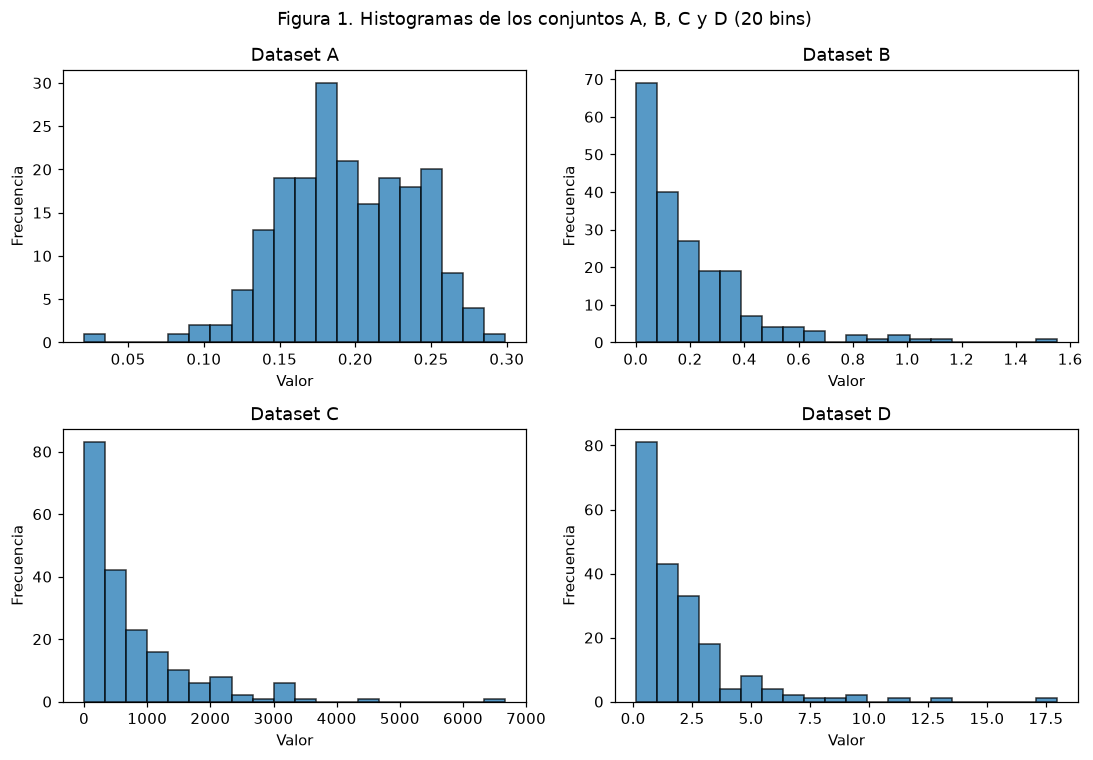
\includegraphics[width=.92\textwidth]{histogramas.png}
\caption{Histogramas de los conjuntos de datos A, B, C y D (20 bins).}\label{fig:hist}
\end{figure}

\paragraph{¿Qué se puede analizar de las medidas descriptivas y los histogramas?}
\begin{itemize}
 \item \textbf{A} es el único conjunto casi simétrico: la media (0,195) y la mediana (0,192) casi
 coinciden, la asimetría es $-0{,}29$ y la variabilidad es baja ($CV=0{,}22$). Los valores están
 acotados en $[0{,}021;\,0{,}299]$ y el histograma tiene forma de campana, lo que apunta a una
 Normal o a una Gamma o Weibull con forma grande. El mínimo está aislado del resto.
 \item \textbf{B} tiene media 0,205 mayor que la mediana 0,138, asimetría 2,41 y $CV=1{,}12\approx1$.
 La moda está en cero y la frecuencia decae de forma monótona: es el perfil de una exponencial.
 \item \textbf{C} tiene una escala muy distinta, de 0,93 a 6670. La media (762) supera mucho a la
 mediana (456), con asimetría 2,48, curtosis 9,1 y $CV=1{,}21>1$: la cola derecha es más
 pesada que la de una exponencial.
 \item \textbf{D} tiene media 2,06 frente a mediana 1,41, asimetría 3,16 y la mayor curtosis
 (14,1), con $CV=1{,}13$. El mínimo es positivo (0,11) y hay valores aislados de hasta 18. Una cola
 tan larga es típica de la Lognormal o la Log-logística.
 \item A y B tienen casi la misma media ($\approx0{,}2$) pero distribuciones opuestas, así que la
 media y la varianza no bastan para elegir un modelo de entrada. Todos los conjuntos son
 positivos, lo que pone en duda la Normal para B, C y D, que tienen asimetría fuerte.
\end{itemize}

\subsection{Análisis de independencia y estabilidad}
Las Figuras~\ref{fig:supA} a~\ref{fig:supD} muestran las cinco gráficas pedidas para cada
conjunto, más la serie de valores frente a su orden. La Tabla~\ref{tab:pruebas} resume las
pruebas numéricas.

\begin{figure}[H]\centering
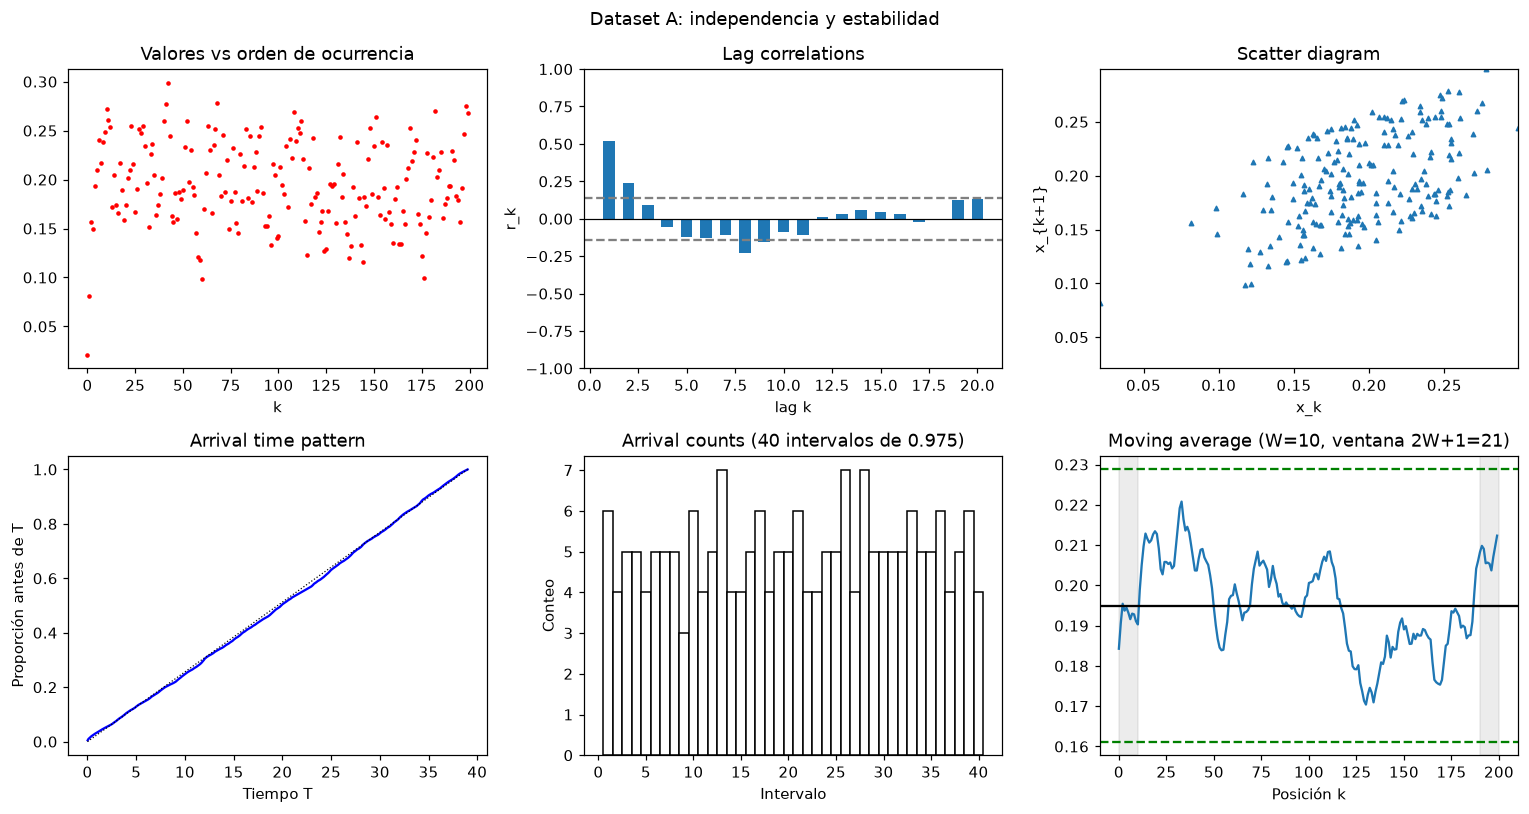
\includegraphics[width=\textwidth]{supuestos_A.png}
\caption{Dataset A: valores frente al orden, correlaciones de retraso, diagrama de dispersión,
patrón de llegadas, conteos por intervalo y media móvil.}\label{fig:supA}
\end{figure}

\paragraph{Dataset A: correlacionado y estacionario.} Las correlaciones $r_1=0{,}517$ y
$r_2=0{,}239$ están muy por encima de la banda y decaen con el retraso, como en un proceso
autorregresivo; también hay valores negativos fuera de la banda en los lags 8 y 9. El diagrama de
dispersión se inclina hacia la diagonal: a un valor alto le sigue otro alto. En cambio, el
patrón de llegadas es prácticamente una recta, los conteos oscilan entre 3 y 7 sin tendencia y
la media móvil se mantiene dentro de las bandas alrededor de 0,195. Sus oscilaciones son lentas,
otra huella de la correlación positiva. Los dos primeros valores (0,021 y 0,081) son bajos y la
serie sube en pocos pasos, lo que sugiere un estado inicial del proceso.

\begin{figure}[H]\centering
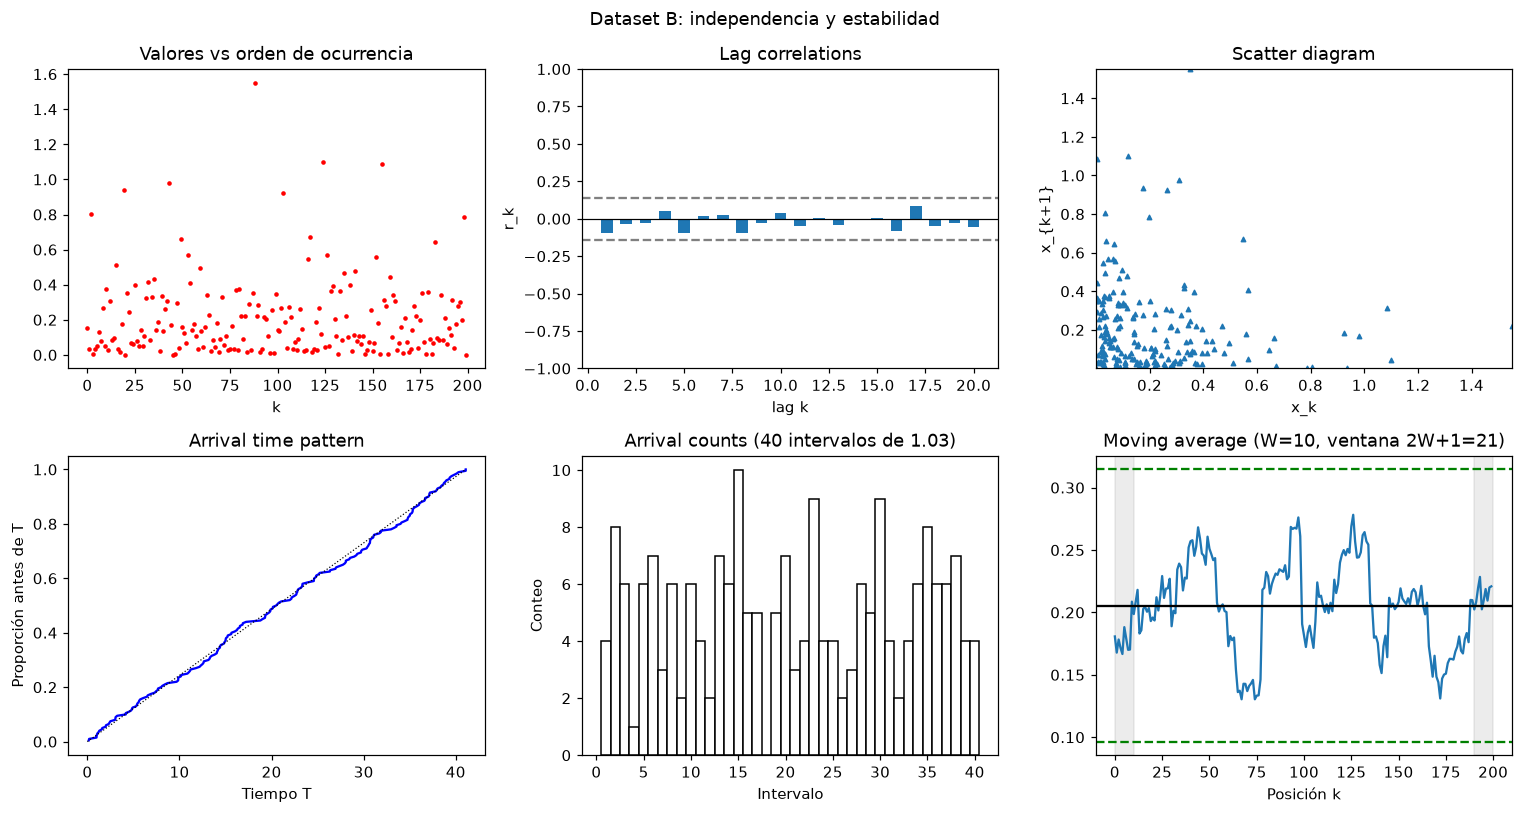
\includegraphics[width=\textwidth]{supuestos_B.png}
\caption{Dataset B: gráficas de independencia y estabilidad.}\label{fig:supB}
\end{figure}

\paragraph{Dataset B: independiente y estacionario.} Todas las correlaciones están dentro de la
banda ($r_1=-0{,}09$), con signos alternados y sin patrón. El diagrama de dispersión es una nube
concentrada cerca del origen, con la forma de la marginal y sin inclinación. El patrón de
llegadas sigue la diagonal, los conteos (0 a 10, media $\approx5$) tienen la dispersión esperable
en un proceso de Poisson y la media móvil oscila entre 0,13 y 0,28 sin tendencia.

\begin{figure}[H]\centering
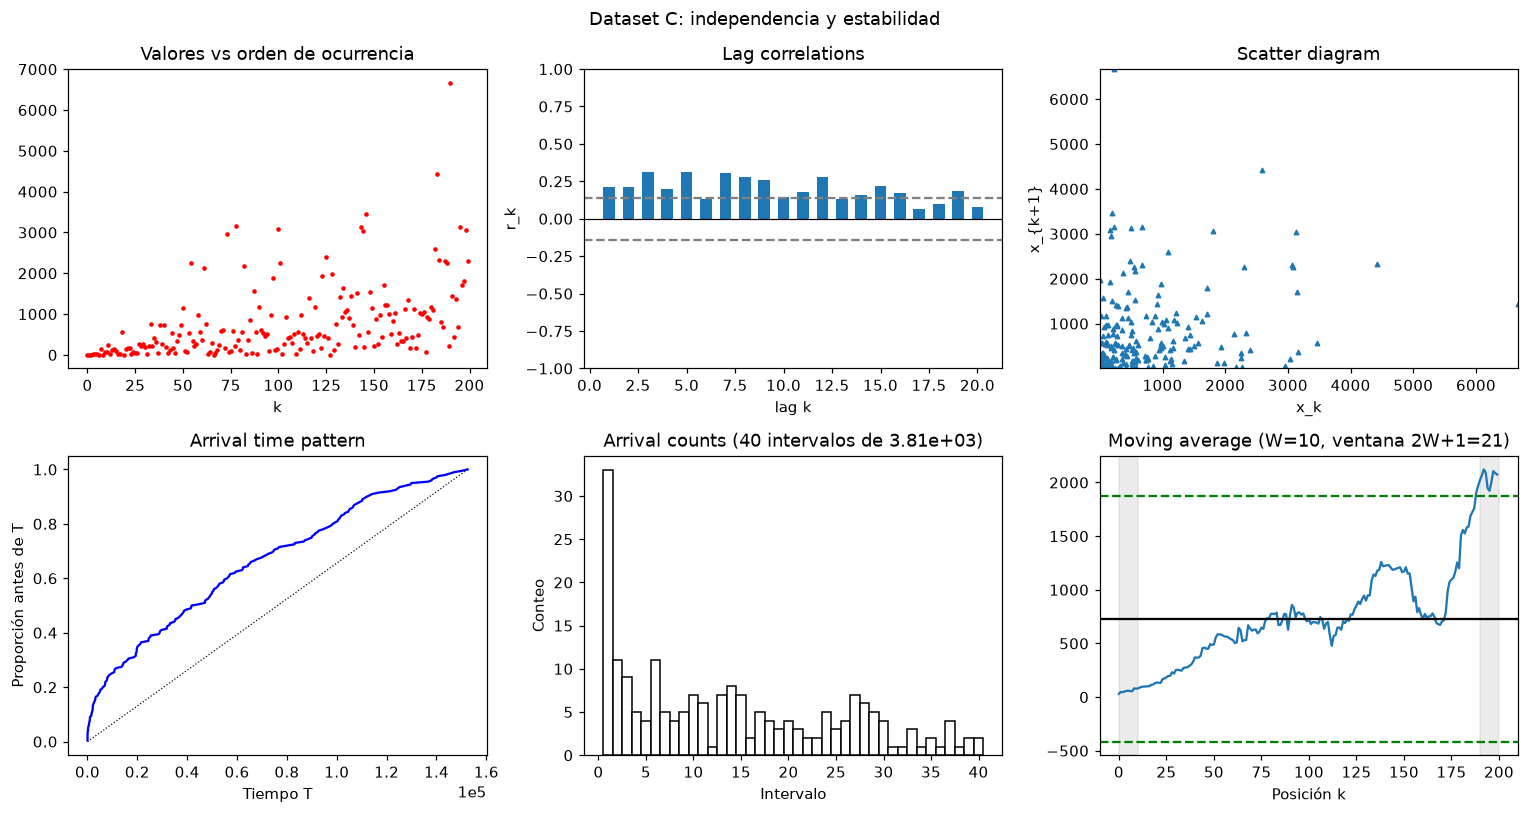
\includegraphics[width=\textwidth]{supuestos_C.png}
\caption{Dataset C: gráficas de independencia y estabilidad.}\label{fig:supC}
\end{figure}

\paragraph{Dataset C: no estacionario.} Los valores crecen con el orden de observación: los 20
primeros no pasan de 565 y los últimos llegan a miles. Todas las correlaciones son positivas y
superan la banda hasta el lag 15 aproximadamente, sin decaer, que es el síntoma típico de una
\emph{tendencia} y no de una dependencia de corto plazo. El patrón de llegadas es una curva
cóncava muy alejada de la diagonal: el 20\,\% de las llegadas ocurre en el 4\,\% del tiempo y la
mitad en el 27\,\%. Los conteos pasan de 33 en el primer intervalo a entre 1 y 8 en los demás, y
la media móvil sube casi sin pausa de 30 a 2100, saliéndose de las bandas al final.

\begin{figure}[H]\centering
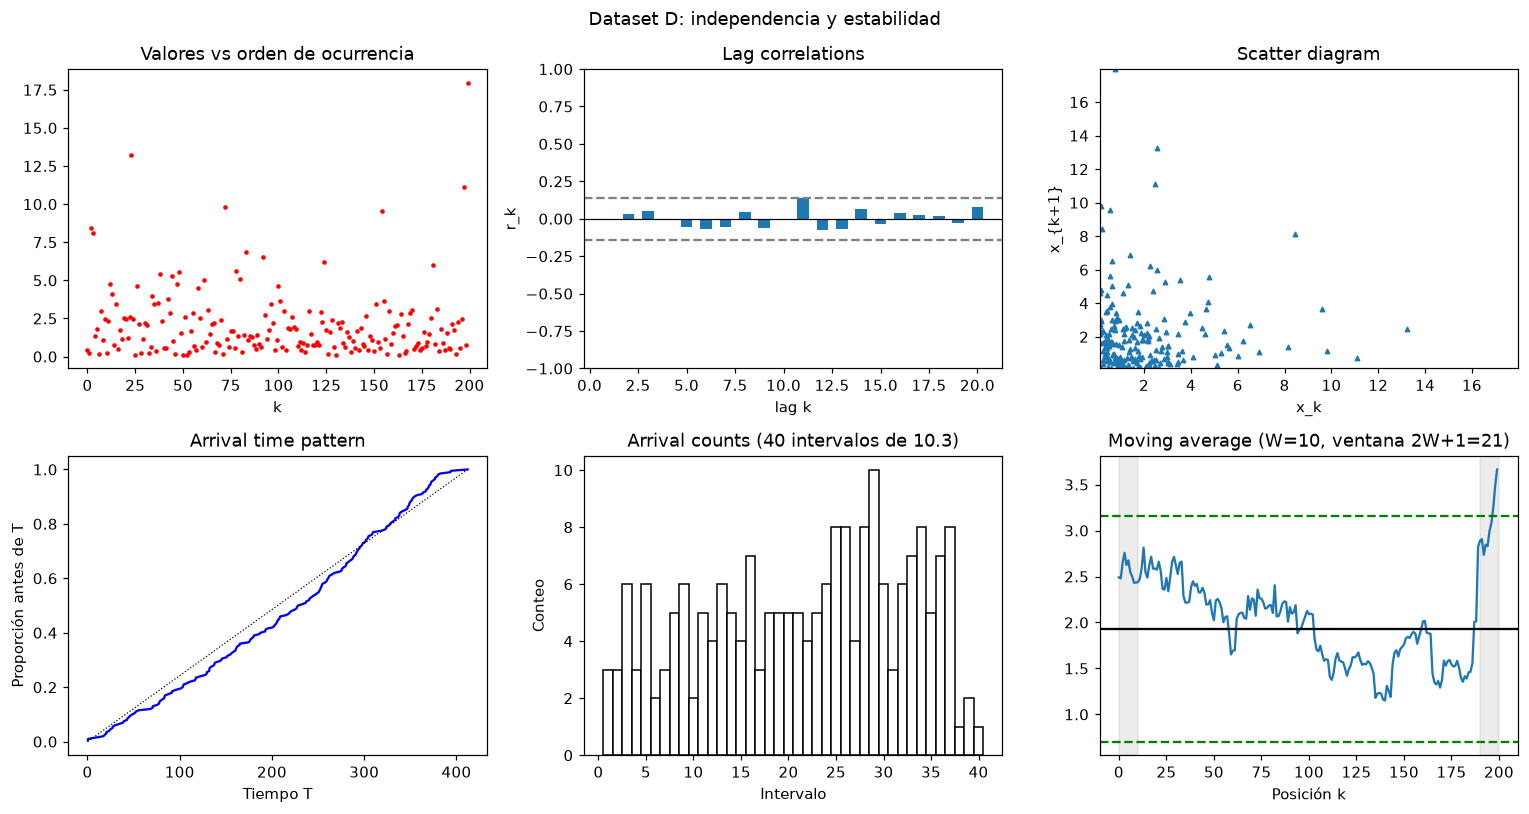
\includegraphics[width=\textwidth]{supuestos_D.png}
\caption{Dataset D: gráficas de independencia y estabilidad.}\label{fig:supD}
\end{figure}

\paragraph{Dataset D: independiente, con estacionariedad aceptable.} Las correlaciones están
dentro de la banda ($r_1=-0{,}003$) y el diagrama de dispersión no tiene inclinación. El patrón de
llegadas queda algo por debajo de la diagonal en la primera mitad (llegadas un poco más lentas) y
luego la cruza. Los conteos van de 2 a 10, algo más altos entre los intervalos 25 y 37. La media
móvil baja suavemente de 2,6 a 1,5 y solo se sale de la banda en el extremo sombreado, donde
pesan los valores 11,1 y 18,0, dos de los tres últimos de la serie. Esta deriva no es
estadísticamente significativa.

\begin{table}[H]\centering\small
\caption{Pruebas de independencia y estabilidad (valores $p$ al nivel 5\,\%). LB: Ljung-Box con
10 lags; $\rho_S$: correlación de Spearman entre valor y orden; K-W: Kruskal-Wallis entre cuatro
bloques de 50 datos.}\label{tab:pruebas}
\setlength{\tabcolsep}{3.5pt}\footnotesize
\begin{tabular}{ccccccc>{\raggedright\arraybackslash}p{.24\textwidth}}\toprule
&$r_1$&$p$ LB&$p$ rachas&$\rho_S$&$p$ Spearman&$p$ K-W&\textbf{Medias por bloque}\\\midrule
\inputtablerows{tablas/tabla_pruebas.tex}
\bottomrule
\end{tabular}\end{table}

\begin{table}[H]\centering\small
\caption{Resumen de la evaluación de supuestos.}\label{tab:resumen_iid}
\begin{tabular}{cp{.33\textwidth}p{.33\textwidth}c}\toprule
\textbf{Dataset}&\textbf{Independencia}&\textbf{Estabilidad}&\textbf{¿IID?}\\\midrule
A&No: $r_1=0{,}52$, LB y rachas rechazan&Sí: sin tendencia ($p$ Spearman $=0{,}14$)&No\\
B&Sí: $p$ LB $=0{,}69$&Sí: $p$ Spearman $=0{,}96$, $p$ K-W $=0{,}99$&Sí\\
C&No (efecto de la tendencia)&No: $\rho_S=0{,}60$; medias por bloque de 191 a 1251&No\\
D&Sí: $p$ LB $=0{,}93$&Sí: deriva leve no significativa ($p=0{,}10$)&Sí\\\bottomrule
\end{tabular}\end{table}

\paragraph{¿Qué se puede determinar sobre la independencia y la estabilidad?} Solo B y D cumplen
los supuestos IID y admiten directamente una distribución univariada. A es estacionario pero
correlacionado, así que generar valores independientes de su distribución marginal haría perder
la persistencia de la serie, y eso afecta, por ejemplo, la formación de colas. C no es
estacionario: su distribución cambia con el tiempo y un único modelo para todos los datos mezcla
escalas distintas. La prueba de rachas de B ($p=0{,}033$) es un resultado aislado: ninguna
correlación sale de la banda y Ljung-Box no rechaza, y con cuatro pruebas por conjunto al 5\,\%
es esperable algún rechazo por azar.

\subsection{Ajuste de curvas y bondad de ajuste}
Las Tablas~\ref{tab:ajA} a~\ref{tab:ajD} presentan los parámetros estimados y los criterios para
las nueve distribuciones, en el orden de la guía. En negrita aparece el mejor valor de cada
criterio, y la última columna da el puesto en el ranking combinado. Los parámetros siguen la
convención de \texttt{scipy.stats}: \emph{escala} es la media en la Exponencial y
$e^{\mu_{\ln}}$ en la Lognormal, $\sigma$ es la desviación estándar de $\ln X$, $a$ y $c$ son
parámetros de forma, y $\text{loc}=0$ se omite.

\newcommand{\tablaajuste}[3]{%
\begin{table}[H]\centering\small
\caption{Bondad de ajuste para el conjunto de datos #1.}\label{#3}
\setlength{\tabcolsep}{4pt}
\begin{tabular}{l>{\raggedright\arraybackslash}p{.33\textwidth}cccc}\toprule
\textbf{Distribución}&\textbf{Parámetros}&\textbf{SSE}&\textbf{AIC}&\textbf{BIC}&\textbf{Puesto}\\\midrule
\inputtablerows{#2}
\bottomrule
\end{tabular}\end{table}}

\tablaajuste{A}{tablas/tabla_ajuste_A.tex}{tab:ajA}
\begin{figure}[H]\centering
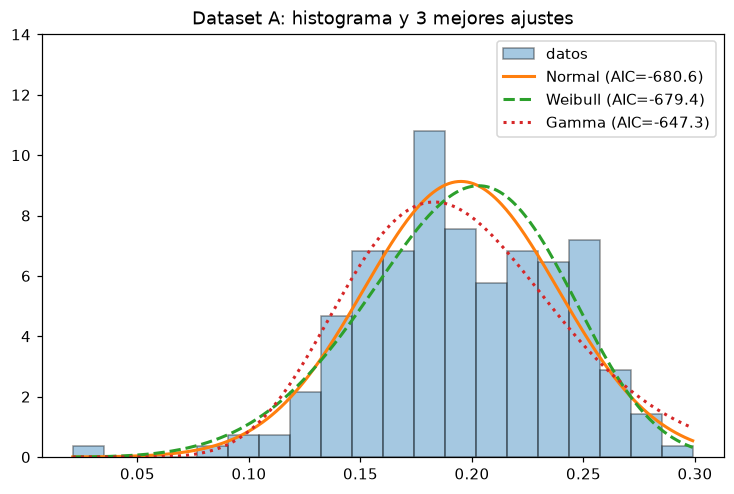
\includegraphics[width=.72\textwidth]{top3_A.png}
\caption{Dataset A: histograma y las tres distribuciones con mejor ajuste.}\label{fig:top3A}
\end{figure}
\paragraph{Dataset A.} La Normal gana en AIC y BIC, con la Weibull ($c=5{,}07$) muy cerca
($\Delta\text{AIC}=1{,}2$). La Gamma tiene el menor SSE, pero su AIC es 33 puntos peor. La
Exponencial y la Rayleigh quedan últimas porque no pueden representar una campana alejada de cero.
La Normal asigna una probabilidad de solo $4\cdot10^{-6}$ a valores negativos, así que en la práctica
no viola el límite físico. Mejores tres: \textbf{Normal, Weibull y Gamma}.

\tablaajuste{B}{tablas/tabla_ajuste_B.tex}{tab:ajB}
\begin{figure}[H]\centering
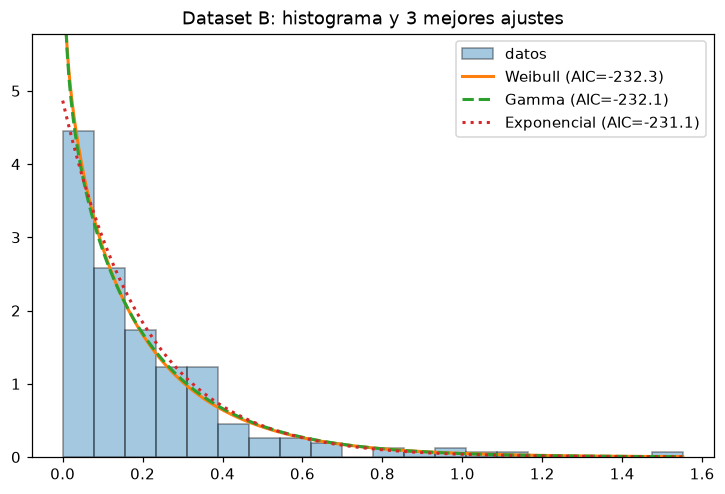
\includegraphics[width=.72\textwidth]{top3_B.png}
\caption{Dataset B: histograma y las tres distribuciones con mejor ajuste.}\label{fig:top3B}
\end{figure}
\paragraph{Dataset B.} La Weibull ($c=0{,}91$), la Gamma ($a=0{,}86$) y la Exponencial (media
0,205) tienen AIC en un rango de 1,1 puntos. La Weibull gana en SSE y AIC, y la Exponencial en
BIC, porque usa un parámetro menos. Las dos formas estimadas están cerca de 1, que es justo el
caso en que Weibull y Gamma se reducen a la Exponencial. Mejores tres: \textbf{Weibull, Gamma y
Exponencial}.

\tablaajuste{C}{tablas/tabla_ajuste_C.tex}{tab:ajC}
\begin{figure}[H]\centering
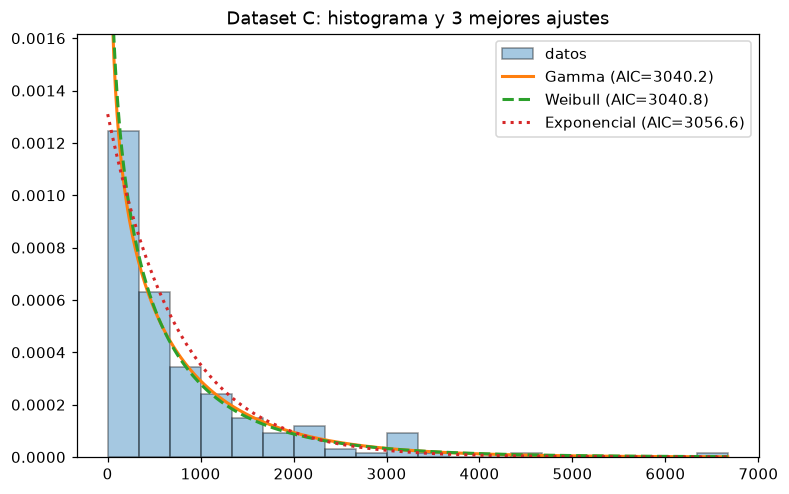
\includegraphics[width=.72\textwidth]{top3_C.png}
\caption{Dataset C: histograma y las tres distribuciones con mejor ajuste.}\label{fig:top3C}
\end{figure}
\paragraph{Dataset C.} La Gamma ($a=0{,}71$) y la Weibull ($c=0{,}80$) empatan en la práctica
($\Delta\text{AIC}=0{,}6$), y la Exponencial queda tercera ($\Delta\text{AIC}=16$). Las formas
menores que 1 reflejan una variabilidad mayor que la exponencial ($CV=1{,}21$). Ese exceso se
explica por la no estacionariedad: mezclar exponenciales con medias distintas produce una
distribución con $CV>1$. El SSE es del orden de $10^{-8}$ porque la densidad de una variable con
escala de miles es muy pequeña, así que no es comparable entre conjuntos. Mejores tres:
\textbf{Gamma, Weibull y Exponencial}.

\tablaajuste{D}{tablas/tabla_ajuste_D.tex}{tab:ajD}
\begin{figure}[H]\centering
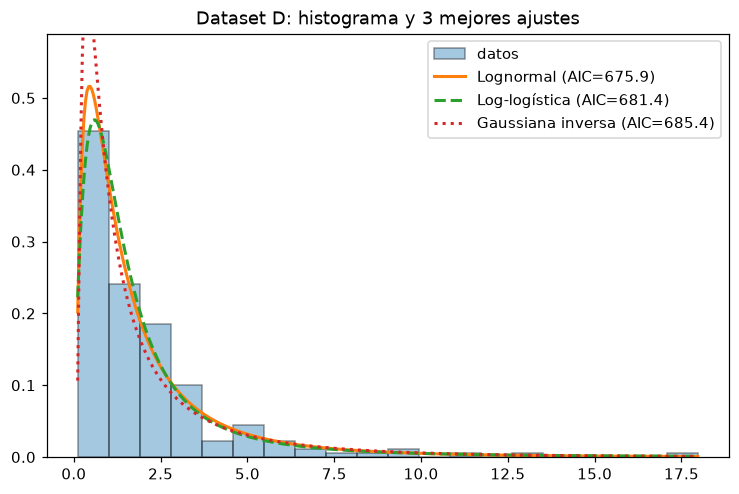
\includegraphics[width=.72\textwidth]{top3_D.png}
\caption{Dataset D: histograma y las tres distribuciones con mejor ajuste.}\label{fig:top3D}
\end{figure}
\paragraph{Dataset D.} La Lognormal gana en AIC y BIC. Sus parámetros equivalen a que
$\ln X$ siga una $N(0{,}241;\,1{,}019^2)$. La Log-logística tiene el menor SSE y queda segunda
($\Delta\text{AIC}=5{,}5$). La Gaussiana inversa es tercera: empata en el ranking con la
Exponencial, pero la supera en AIC y BIC. Las tres tienen moda positiva y cola derecha larga,
como el histograma. Mejores tres: \textbf{Lognormal, Log-logística y Gaussiana inversa}.

\paragraph{Verificación del mejor modelo.} En los cuatro conjuntos, los gráficos P-P quedan
pegados a la diagonal (Figuras~\ref{fig:ppqq1} y~\ref{fig:ppqq2}), y Kolmogorov-Smirnov no rechaza
el mejor modelo: $p=0{,}63$ (A), $0{,}96$ (B), $0{,}91$ (C) y $0{,}59$ (D). En el Q-Q de A, el
primer dato (0,021) queda muy por debajo del modelo, y la cola derecha de los datos es algo más
corta que la normal. En el de D, la Lognormal predice extremos algo mayores que los observados:
al máximo, 18,0, le corresponde un cuantil teórico de $\approx22$. Para B, la razón de
verosimilitudes \textbf{no rechaza} que la forma sea 1: Exponencial frente a Weibull, $p=0{,}077$,
y frente a Gamma, $p=0{,}085$. El buen K-S de C solo indica que la distribución agregada se
parece a una Gamma; no valida el supuesto IID, que ya falló.

\begin{figure}[H]\centering
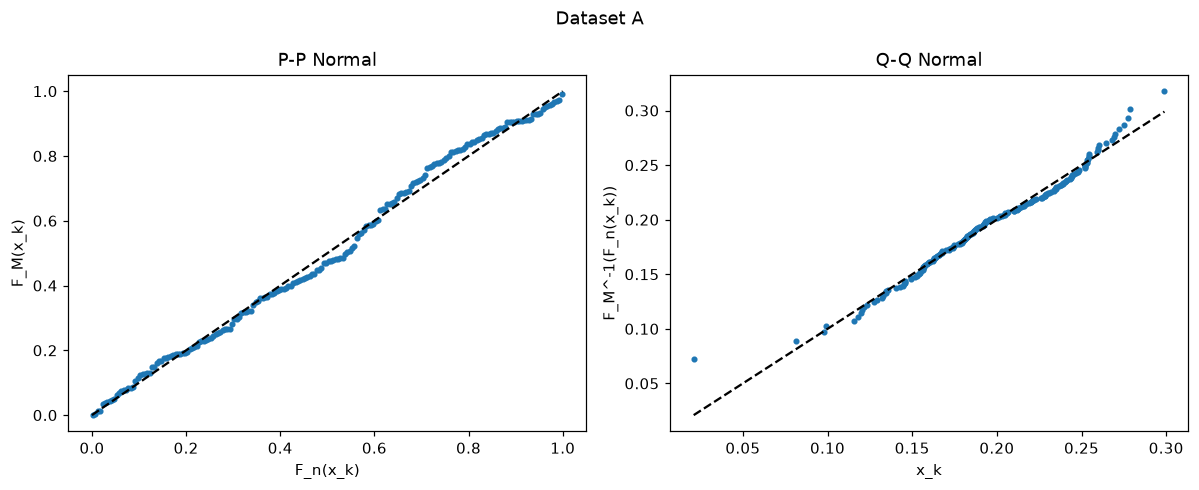
\includegraphics[width=.9\textwidth]{ppqq_A.png}\\[2pt]
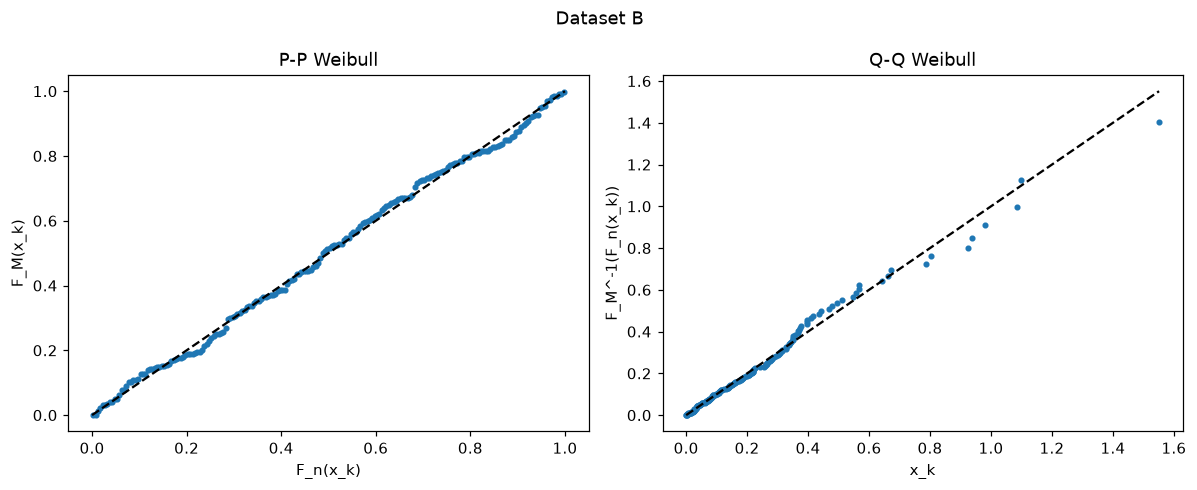
\includegraphics[width=.9\textwidth]{ppqq_B.png}
\caption{Gráficos P-P y Q-Q del mejor modelo para los conjuntos A (Normal) y B (Weibull).}\label{fig:ppqq1}
\end{figure}
\begin{figure}[H]\centering
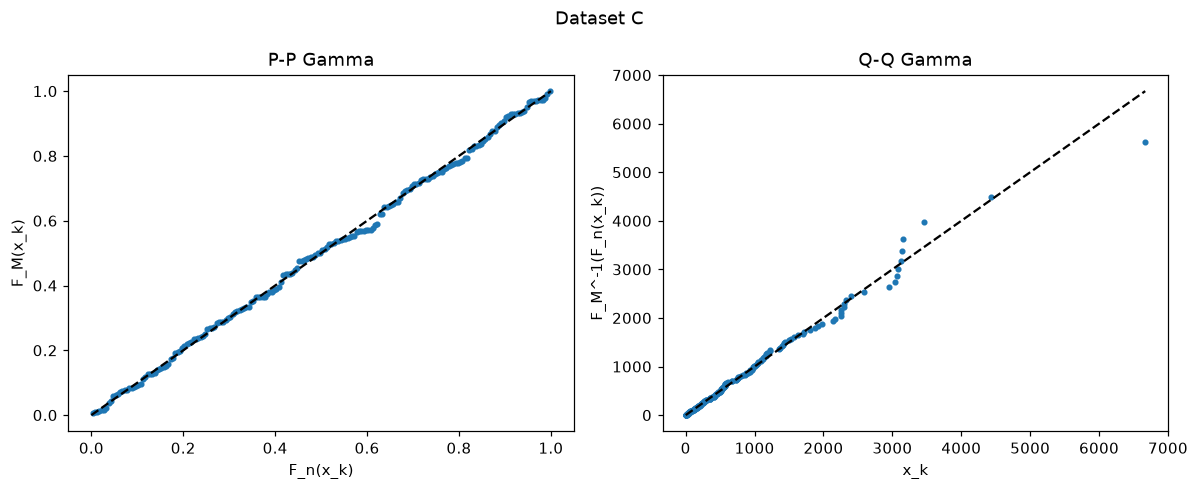
\includegraphics[width=.9\textwidth]{ppqq_C.png}\\[2pt]
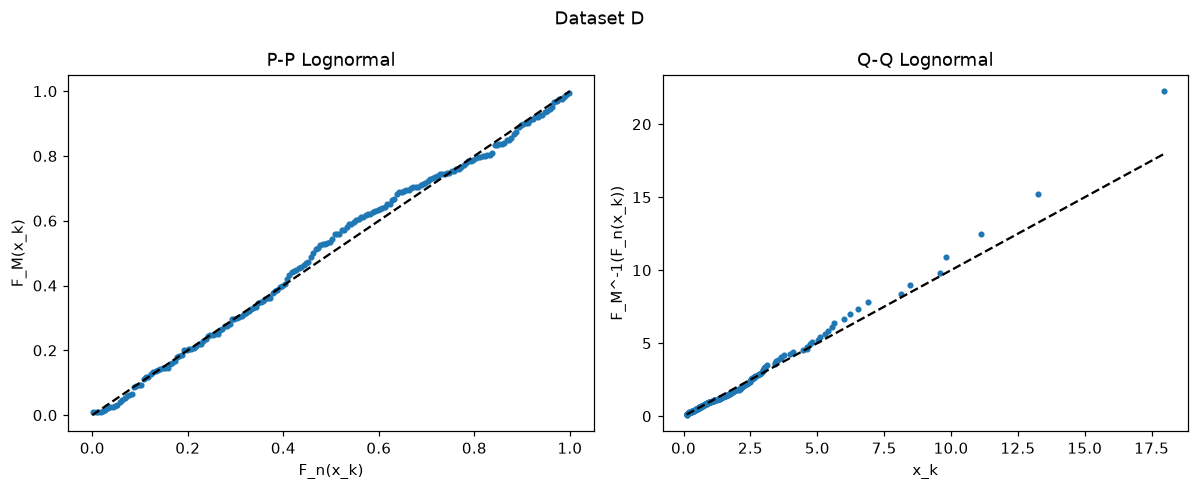
\includegraphics[width=.9\textwidth]{ppqq_D.png}
\caption{Gráficos P-P y Q-Q del mejor modelo para los conjuntos C (Gamma) y D (Lognormal).}\label{fig:ppqq2}
\end{figure}

\subsection{Modelos para los conjuntos no IID}
\paragraph{Dataset A: AR(1).} Con $\hat\mu=0{,}195$ y $\hat\varphi=r_1=0{,}517$, los residuos
$\varepsilon_k=(x_k-\hat\mu)-\hat\varphi(x_{k-1}-\hat\mu)$ ya no están correlacionados (Ljung-Box
$p=0{,}29$). Sin embargo, \emph{no son normales}: tienen curtosis $-1{,}24$ y un rango cerrado de
$\pm0{,}06$, que es la firma de una uniforme. El ajuste $U(-0{,}060;\,0{,}061)$ tiene K-S
$p=0{,}73$ y un AIC 81 puntos mejor que el de la normal. El modelo de entrada es entonces
\begin{equation}
 X_k=0{,}195+0{,}517\,(X_{k-1}-0{,}195)+\varepsilon_k,\qquad \varepsilon_k\sim U(-0{,}060;\,0{,}061).
\end{equation}
Su marginal es una suma ponderada de uniformes, casi normal pero de colas cortas, lo que coincide
con el Q-Q de la Normal.

\begin{figure}[H]\centering
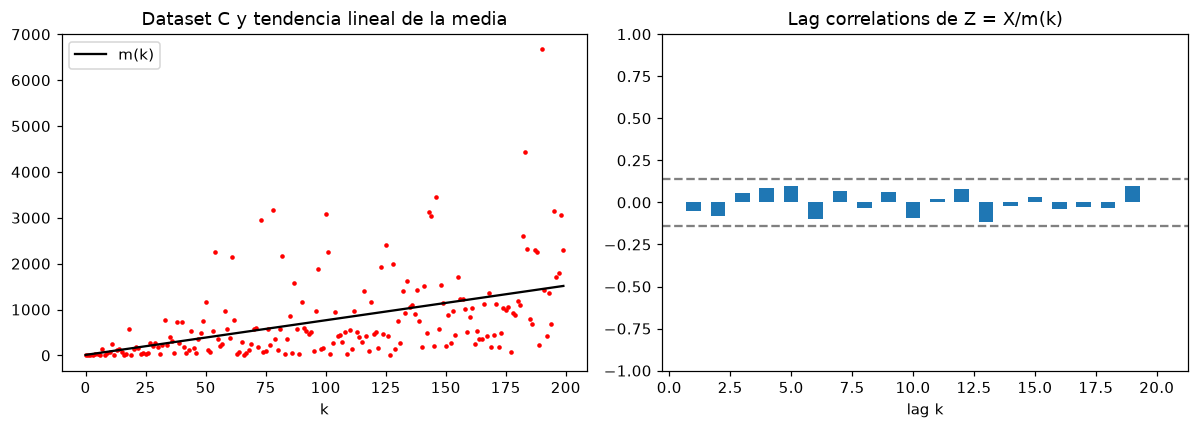
\includegraphics[width=\textwidth]{tendencia_C.png}
\caption{Dataset C: tendencia lineal de la media (izquierda) y correlaciones de retraso de los
datos normalizados $Z_k=X_k/m(k)$ (derecha).}\label{fig:tendC}
\end{figure}

\paragraph{Dataset C: media con tendencia.} La recta de mínimos cuadrados
$m(k)=10{,}82+7{,}553\,k$ tiene pendiente significativa ($p\approx10^{-12}$). Los datos
normalizados $Z_k=X_k/m(k)$ son IID (Figura~\ref{fig:tendC}): $r_1=-0{,}05$, Ljung-Box $p=0{,}30$
y Kruskal-Wallis $p=0{,}87$. Además son exponenciales: $CV=1{,}04$, la Exponencial gana en AIC y
BIC, la Gamma y la Weibull estimadas tienen forma $\approx1$ ($a=1{,}03$, $c=1{,}01$) y K-S da
$p=0{,}84$. Es decir, C son tiempos entre llegadas exponenciales con media creciente: un proceso de
llegadas cuya tasa disminuye con el tiempo.

\subsection{Selección de la distribución}
\begin{table}[H]\centering\small
\caption{Distribución seleccionada y modelo de entrada recomendado por conjunto de datos.}\label{tab:seleccion}
\begin{tabular}{c>{\raggedright\arraybackslash}p{.3\textwidth}>{\raggedright\arraybackslash}p{.5\textwidth}}\toprule
\textbf{Dataset}&\textbf{Distribución (top 3)}&\textbf{Modelo para la simulación}\\\midrule
A&Normal($\mu=0{,}195$; $\sigma=0{,}0437$)&AR(1): $\varphi=0{,}517$, $\varepsilon\sim U(-0{,}060;\,0{,}061)$\\
B&Exponencial(media $0{,}2054$)&IID Exponencial (tasa 4,87)\\
C&Exponencial con media variable&$X_k=m(k)\,Z_k$, $m(k)=10{,}82+7{,}553\,k$, $Z\sim$ Exp(media 0,988)\\
D&Lognormal($\sigma=1{,}019$; escala 1,273)&IID Lognormal\\\bottomrule
\end{tabular}\end{table}

\paragraph{¿Cuál de las tres distribuciones con mejor ajuste se selecciona y por qué?}
\begin{itemize}
 \item \textbf{A: Normal.} Gana en AIC y BIC, respeta en la práctica el rango de los datos y su Q-Q
 es muy bueno en el centro. La Weibull es casi equivalente, pero la Normal es más simple de
 interpretar y es la marginal natural de un proceso autorregresivo. Como A está correlacionado,
 en la simulación no deben generarse valores independientes de la Normal, sino el AR(1).
 \item \textbf{B: Exponencial.} Se elige por parsimonia: tiene el mejor BIC, la razón de
 verosimilitudes no justifica el parámetro de forma de la Weibull o la Gamma ($p>0{,}07$) y la
 diferencia de AIC es de solo 1,1. Además es coherente con 5.2: datos IID con patrón de
 llegadas lineal, es decir, llegadas de Poisson.
 \item \textbf{C: Exponencial, con media variable en el tiempo.} Entre las tres mejores, la Gamma
 ajusta mejor los datos agregados, pero solo porque mezcla tramos con escalas distintas. Al
 quitar la tendencia, la Exponencial es la mejor distribución, y es la que debe usarse
 combinada con $m(k)$. Si solo se quisiera reproducir la distribución agregada de estos 200
 datos, se usaría la Gamma ($a=0{,}706$; escala 1080).
 \item \textbf{D: Lognormal.} Es la mejor en AIC y BIC ($\Delta\text{AIC}=5{,}5$ frente a la
 Log-logística), los datos son IID, y P-P, Q-Q y K-S no muestran problemas. Su cola algo más pesada
 que la de los datos es conservadora en un estudio de simulación.
\end{itemize}

\section{Conclusiones}
\begin{itemize}
 \item La estadística descriptiva orienta la elección de familias candidatas: la asimetría y el
 coeficiente de variación separaron de inmediato el conjunto simétrico (A) de los tres con cola
 derecha (B, C y D). Sin embargo, no detecta dependencia ni tendencias.
 \item Las gráficas de 5.2 y las pruebas numéricas son indispensables antes de ajustar: dos de los
 cuatro conjuntos no son IID. A está autocorrelacionado ($r_1=0{,}52$) y C tiene una tendencia
 creciente en la media.
 \item Un buen ajuste de la distribución marginal no valida el supuesto IID. En C, la Gamma pasa
 K-S con $p=0{,}91$, pero el proceso real son exponenciales con media creciente; usar la Gamma con
 valores independientes no reproduciría su evolución en el tiempo.
 \item SSE, AIC y BIC suelen coincidir, pero no siempre. El SSE depende de los bins y de la escala, y
 el AIC y el BIC penalizan los parámetros. Cuando las diferencias son pequeñas, conviene preferir
 el modelo más simple, apoyándose en pruebas como la razón de verosimilitudes (Exponencial en B).
 \item Los modelos recomendados son: AR(1) con innovaciones uniformes para A, Exponencial IID para
 B, Exponencial con media lineal en el tiempo para C y Lognormal IID para D.
\end{itemize}

\begin{thebibliography}{9}
\bibitem{banks1998} J. Banks (ed.), \textit{Handbook of Simulation: Principles, Methodology,
Advances, Applications, and Practice}. John Wiley \& Sons, 1998, cap. 3.
\bibitem{amat2021} J. Amat Rodrigo, \textit{Ajuste y selección de distribuciones con Python},
2021, licencia CC BY-NC-SA 4.0.
\url{https://www.cienciadedatos.net/documentos/pystats01-ajuste-distribuciones-python.html}.
DOI: \href{https://doi.org/10.5281/zenodo.10006330}{10.5281/zenodo.10006330}.
\bibitem{scipy} P. Virtanen et al., ``SciPy 1.0: fundamental algorithms for scientific computing
in Python'', \textit{Nature Methods}, 17, 261--272, 2020.
\end{thebibliography}
\end{document}
